
\begin{figure*}[t!]
    \centering
    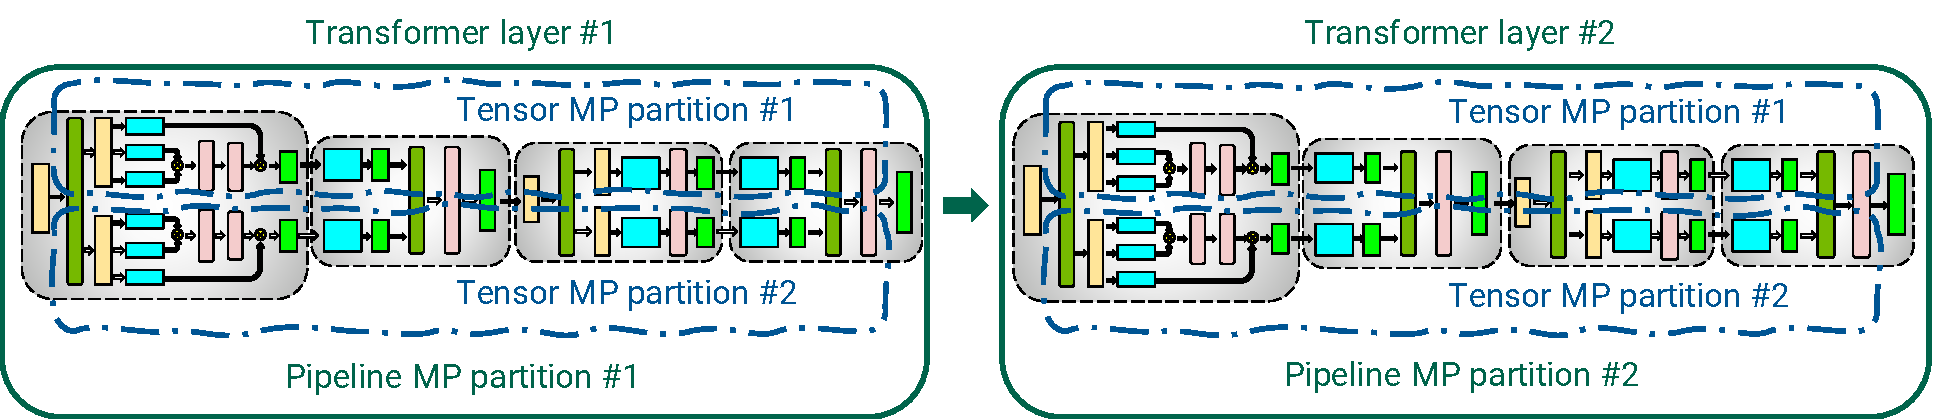
\includegraphics[keepaspectratio=1.0,width=0.9\textwidth]{figures/tensor_plus_pipeline_model_parallelism.pdf}
    \vspace{-0.1in}
    \caption{
       Combination of tensor and pipeline model parallelism (MP) used in this work for transformer-based models.
    }
    \label{fig:tensor_plus_pipeline_model_parallelism}
    \vspace{-0.15in}
\end{figure*}

\begin{figure*}[t!]
    \centering
    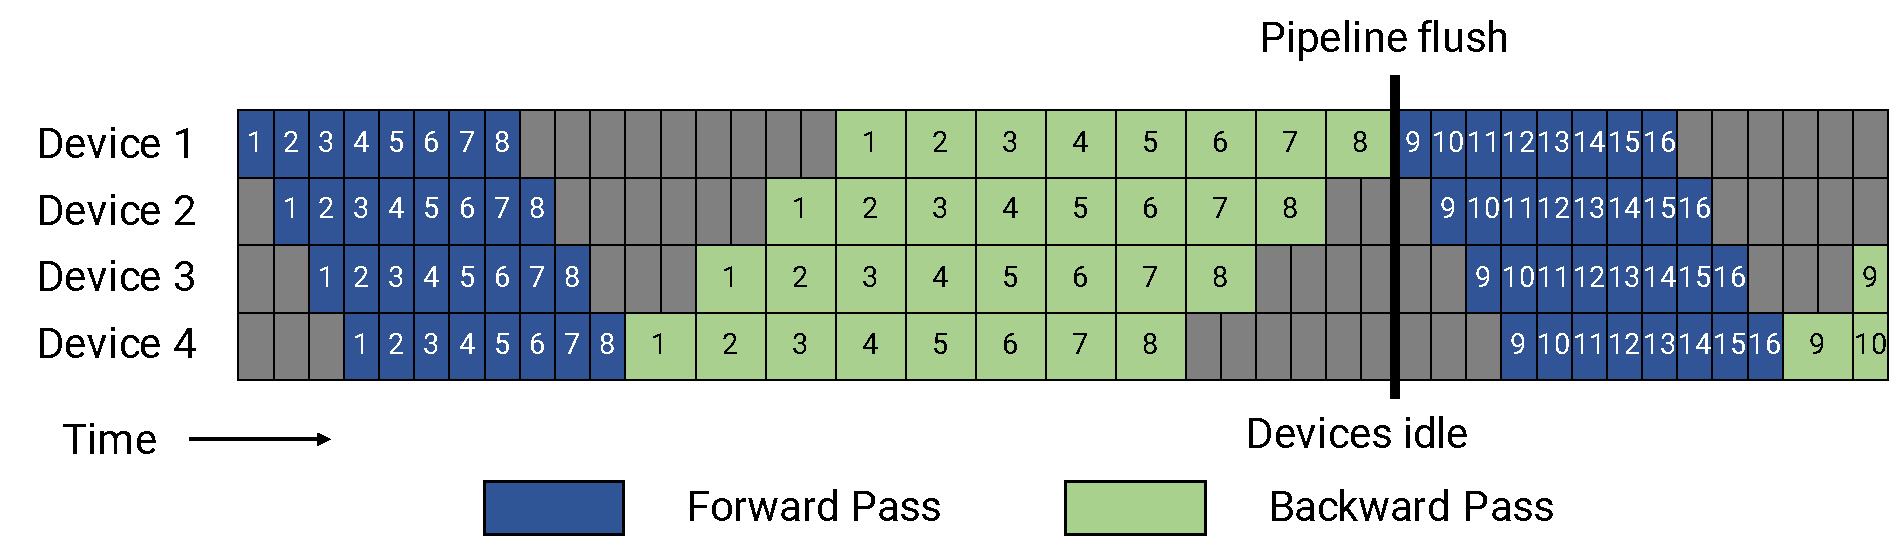
\includegraphics[keepaspectratio=1.0,width=0.75\textwidth]{figures/gpipe.pdf}
    \vspace{-0.1in}
    \caption{
        GPipe pipeline schedule with forward passes (blue) for all microbatches (represented by numbers) followed by backward passes (green). The gray area represents the pipeline bubble. For simplicity, we assume that the backward pass takes twice as long as the forward pass. The efficiency of the pipeline schedule does not depend on this factor. Each batch in this example consists of 8 microbatches, and the numbers in each blue or green box are unique identifiers given to the corresponding microbatch (in particular, the first batch consists of microbatches $1-8$, the second batch consists of microbatches $9-16$, and so on). The optimizer is stepped and weight parameters updated at the pipeline flush to ensure strict optimizer semantics, leading to idle devices and a pipeline bubble.
    }
    \label{fig:gpipe}
\end{figure*}

\begin{figure*}[t!]
    \centering
    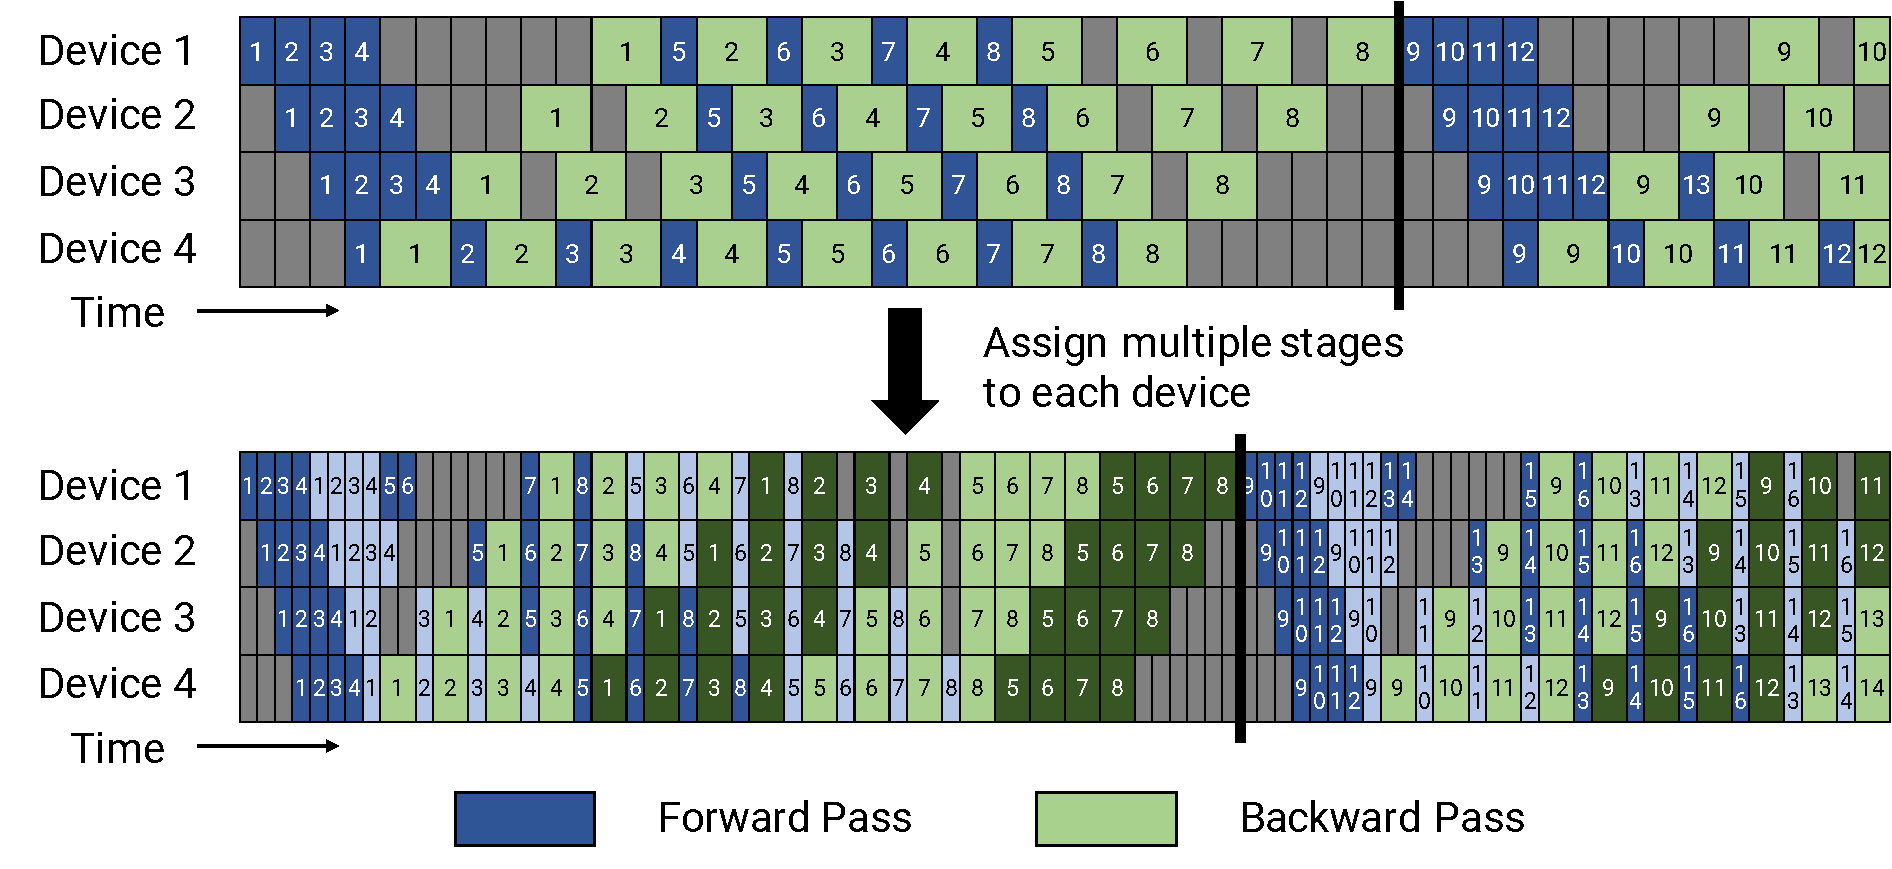
\includegraphics[keepaspectratio=1.0,width=0.74\textwidth]{figures/interleaved_schedule.pdf}
    \vspace{-0.1in}
    \caption{
        Default and interleaved 1F1B pipeline schedules. The top figure shows the default non-interleaved 1F1B schedule. The bottom figure shows the interleaved 1F1B schedule, where each device is assigned multiple chunks (in this case, 2). Dark colors show the first chunk and light colors show the second chunk. The size of the pipeline bubble is smaller (the pipeline flush happens sooner in the interleaved timeline).
    }
    \label{fig:interleaved_schedule}
\end{figure*}
\section{Modes of Parallelism}
\label{sec:model_parallelism}

In this section, we discuss the parallelism techniques that facilitate the \emph{efficient} training of large models that do not fit in the memory of a single GPU. In this work, we combine pipeline model parallelism and tensor model parallelism (combination shown in Figure~\ref{fig:tensor_plus_pipeline_model_parallelism}) with data parallelism. We call this PTD-P for short.

\subsection{Data Parallelism}

With data parallelism~\cite{xing2015petuum, pytorchdistributed}, each worker has a copy of the full model, the input dataset is sharded, and workers aggregate their gradients periodically to ensure that all workers see a consistent version of the weights. For large models which do not fit on a single worker, data parallelism can be used on smaller model shards.

\subsection{Pipeline Model Parallelism}

With pipeline parallelism, the layers of a model are sharded across multiple devices. When used on models with the same transformer block repeated, each device can be assigned an equal number of transformer layers. We do not consider more asymmetric model architectures, where assignment of layers to pipeline stages is harder; we defer to related work~\cite{narayanan2019pipedream, flexflow, tarnawski2020efficient} to solve this problem.

A batch is split into smaller microbatches; execution is then pipelined across microbatches. Pipelining schemes need to ensure that inputs see consistent weight versions across forward and backward passes for well-defined synchronous weight update semantics. Specifically, naive pipelining can lead to an input seeing weight updates in the backward pass not seen in the forward pass.

To retain strict optimizer semantics \emph{exactly}, we introduce periodic pipeline flushes so that optimizer steps are synchronized across devices. At the start and end of every batch, devices are idle. We call this idle time the \emph{pipeline bubble}, and want to make it as small as possible. Asynchronous and bounded-staleness approaches such as PipeMare, PipeDream, and PipeDream-2BW~\cite{yang2021pipemare, pb2021kosson, narayanan2019pipedream, narayanan2021memory} do away with flushes completely, but relax weight update semantics. We defer consideration of such schemes to future work.

There are several possible ways of scheduling forward and backward microbatches across devices; each approach offers different tradeoffs between pipeline bubble size, communication, and memory footprint. We discuss two such approaches in this section.


\subsubsection{Default Schedule}
\label{sec:pipeline_parallelism_bubble}
GPipe~\cite{huang2019gpipe} proposes a schedule where the forward passes for all microbatches in a batch are first executed, followed by backward passes for all microbatches (shown in Figure~\ref{fig:gpipe}). We can quantify the size of GPipe's pipeline bubble ($t_{pb}$). We denote the number of microbatches in a batch as $m$, the number of pipeline stages (number of devices used for pipeline parallelism) as $p$, the ideal time per iteration as $t_{id}$ (assuming perfect or ideal scaling), and the time to execute a single microbatch’s forward and backward pass as $t_f$ and $t_b$. In this schedule, the pipeline bubble consists of $p-1$ forward passes at the start of a batch, and $p-1$ backward passes at the end. The total amount of time spent in the pipeline bubble is then $t_{pb}=(p-1)\cdot(t_f+t_b)$. The ideal processing time for the batch is $t_{id}=m\cdot(t_f+t_b)$. Therefore, the fraction of ideal computation time spent in the pipeline bubble is:
$$\text{Bubble time fraction (pipeline bubble size)}=\frac{t_{pb}}{t_{id}}=\frac{p-1}{m}.$$

For the bubble time fraction to be small, we thus need $m \gg p$. However, for such large $m$, this approach has a high memory footprint as it requires stashed intermediate activations (or just input activations for each pipeline stage when using activation recomputation) to be kept in memory for all $m$ microbatches through the lifetime of a training iteration.

Instead, we use the PipeDream-Flush schedule~\cite{narayanan2021memory}. In this schedule, we first enter a warm-up phase where workers perform differing numbers of forward passes as shown in Figure~\ref{fig:interleaved_schedule} (top). This schedule limits the number of in-flight microbatches (the number of microbatches for which the backward pass is outstanding and activations need to be maintained) to the depth of the pipeline, instead of the number of microbatches in a batch. After the warm-up phase, each worker then enters a steady state, where workers perform one forward pass followed by one backward pass (1F1B for short). Finally, at the end of a batch, we complete backward passes for all remaining in-flight microbatches. The time spent in the bubble is the same for this new schedule, but the number of outstanding forward passes is at most the number of pipeline stages for the PipeDream-Flush schedule. As a result, this schedule requires activations to be stashed for $p$ or fewer microbatches (compared to $m$ microbatches for the GPipe schedule). Consequently, when $m \gg p$, PipeDream-Flush is much more memory-efficient than GPipe.


\subsubsection{Schedule with Interleaved Stages}
To reduce the size of the pipeline bubble, each device can perform computation for multiple subsets of layers (called a model chunk), instead of a single contiguous set of layers. For example, if each device had 4 layers before (i.e., device 1 had layers $1-4$, device 2 had layers $5-8$, and so on), we could have each device perform computation for two model chunks (each with 2 layers), i.e., device 1 has layers $1,2,9,10$; device 2 has layers $3,4,11,12$; and so on. With this scheme, each device in the pipeline is assigned multiple pipeline stages (each pipeline stage has less computation compared to before).

As before, we can use an ``all-forward, all-backward'' version of this schedule, but this has a high memory footprint (proportional to $m$). Instead, we developed an interleaved schedule that adapts the memory-efficient 1F1B schedule from before. This new schedule is shown in Figure~\ref{fig:interleaved_schedule}, and requires the number of microbatches in a batch to be an integer multiple of the degree of pipeline parallelism (number of devices in the pipeline). For example, with 4 devices, the number of microbatches in a batch must be a multiple of 4.

As shown in Figure~\ref{fig:interleaved_schedule}, the pipeline flush for the same batch size happens sooner in the new schedule. If each device has $v$ stages (or model chunks), then the forward and backward time for a microbatch for each stage or chunk will now be $t_f/v$ and $t_b/v$. The pipeline bubble time thus reduces to $t^{\text{int.}}_{pb} = \frac{(p-1)\cdot(t_f+t_b)}{v}$, and the bubble time fraction is then:
$$\text{Bubble time fraction (pipeline bubble size)}=\frac{t^{\text{int.}}_{pb}}{t_{id}}=\frac{1}{v} \cdot \frac{p-1}{m}.$$

This means that the new schedule reduces the bubble time by $v$. This reduced pipeline bubble size, however, does not come for free: this schedule requires extra communication. Quantitatively, the amount of communication also increases by $v$. In the next section, we discuss how we can utilize the 8 InfiniBand networking cards in a multi-GPU server (e.g., a DGX A100 node) to reduce the impact of this extra communication.


\subsection{Tensor Model Parallelism}
\label{sec:tensor_model_parallelism}

With tensor model parallelism, individual layers of the model are partitioned over multiple devices. In this paper, we use the particular partitioning strategy used by Megatron~\cite{shoeybi2019megatron} for transformer layers, the bedrock of language models. We can apply similar ideas to other types of models, like CNNs, as well. We briefly outline this strategy, illustrated in Figure~\ref{fig:tensor_model_parallelism}, below.

A transformer layer consists of a self-attention block followed by a two-layer multi-layer perceptron (MLP). Further details of the transformer layer can be found in Vaswani et al~\cite{vaswani2017attention}. 

The MLP block consists of two GEMMs and a GeLU non-linearity:
$$Y = \textrm{GeLU}(XA). \, \, \, \, \, Z = \textrm{Dropout}(YB).$$
We can split $A$ along its columns $A=[A_1, A_2]$. This partitioning allows the GeLU non-linearity to be independently applied to the output of each partitioned GEMM:
 \begin{equation}
    [Y_1, Y_2]= [\textrm{GeLU}(XA_1), \textrm{GeLU}(XA_2)].  \nonumber
 \end{equation}
 This is advantageous as it removes the need for synchronization (needed if $A$ is split along its rows since GeLU is non-linear).
 
 The rows of the second weight matrix $B$ can then be split along its rows to remove the need for any communication between the GEMMs (shown in Figure~\ref{fig:tensor_model_parallelism_mlp}), as shown below:
 \begin{equation}
    B=\begin{bmatrix}
        B_1 \\
        B_2
    \end{bmatrix}, \
     Y = [Y_1, Y_2]. \nonumber
 \end{equation}
 The output of the second GEMM is then reduced across the GPUs before the dropout layer.
 
 \begin{figure}[t!]
 \centering
    \begin{subfigure}[c]{\columnwidth}
        \centering
        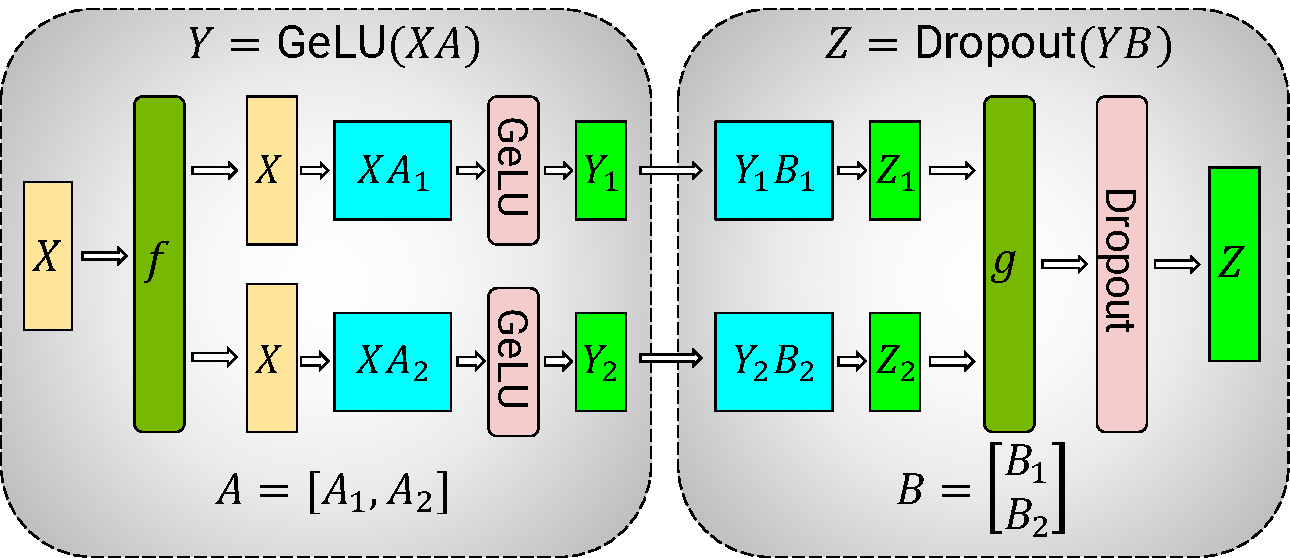
\includegraphics[keepaspectratio=1.0,width=0.85\columnwidth]{figures/mlp_mp_2.pdf}
        \caption{MLP.}
        \label{fig:tensor_model_parallelism_mlp}
    \end{subfigure}
    \begin{subfigure}[c]{\columnwidth}
        \centering
        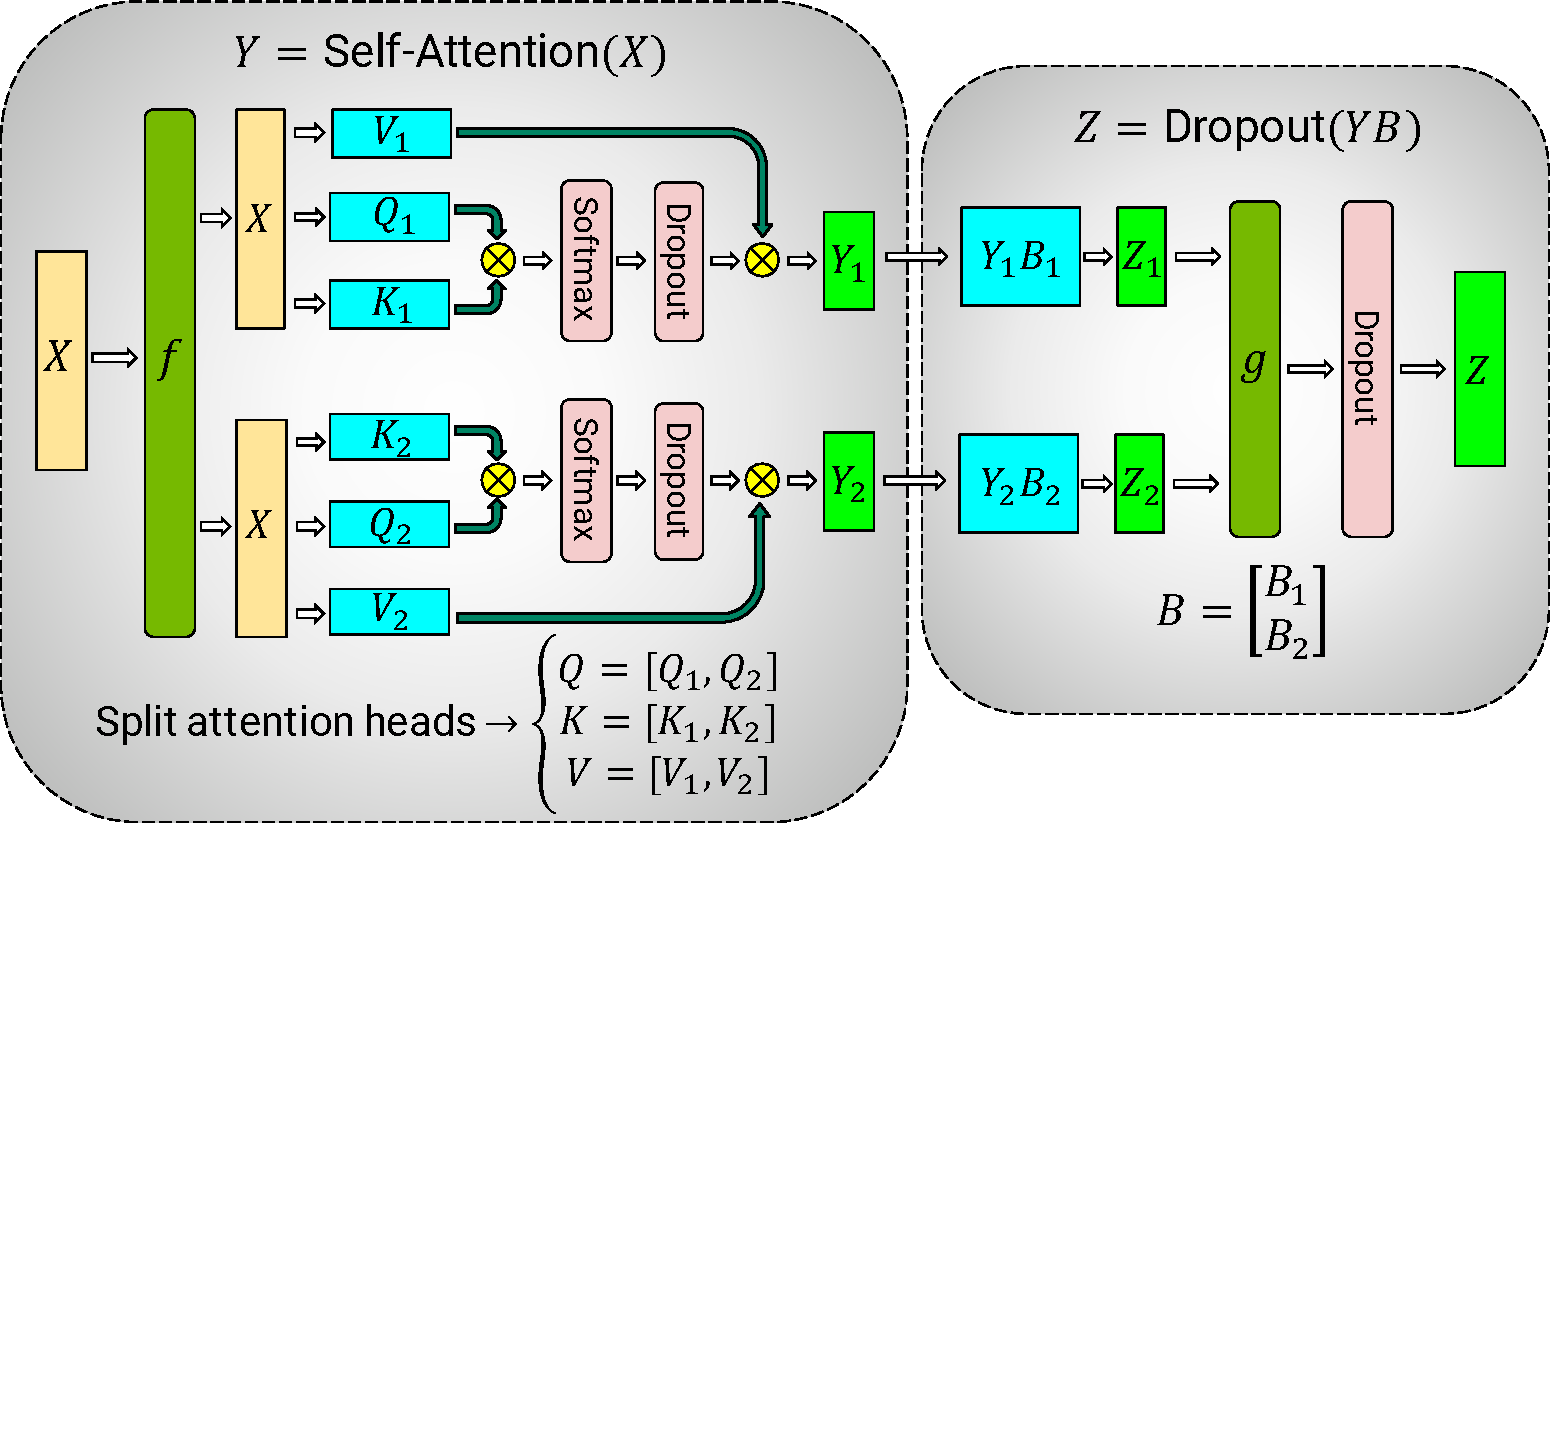
\includegraphics[keepaspectratio=1.0,width=\columnwidth]{figures/attention_mp_2.pdf}
        \vspace{-1.5in}
        \caption{Self-Attention.}
        \label{fig:tensor_model_parallelism_self_attention}
    \end{subfigure}
    \vspace{-0.1in}
    \caption{
        Blocks of transformer model partitioned with tensor model parallelism (figures borrowed from Megatron~\cite{shoeybi2019megatron}). $f$ and $g$ are conjugate. $f$ is the identity operator in the forward pass and all-reduce in the backward pass, while $g$ is the reverse.
    }
    \label{fig:tensor_model_parallelism}
    \vspace{-0.2in}
\end{figure}

We exploit the inherent parallelism in the multi-head attention operation to partition the self-attention block (shown in Figure~\ref{fig:tensor_model_parallelism_self_attention}). The key ($K$), query ($Q$), and value ($V$) matrices can be partitioned in a column-parallel fashion. The output linear layer can then directly operate on the partitioned output of the attention operation (weight matrix partitioned across rows).

This approach splits GEMMs in the MLP and self-attention blocks across GPUs while requiring only two all-reduce operations in the forward pass ($g$ operator) and two all-reduces in the backward pass ($f$ operator). We implemented $f$ and $g$ in a few lines of code.
